\documentclass[11pt,a4paper]{report}
\usepackage[utf8]{inputenc}
\usepackage[french]{babel}
\usepackage[T1]{fontenc}
\usepackage{amsmath}
\usepackage{amsfonts}
\usepackage{amssymb}
\usepackage{graphicx}
\usepackage{lmodern}
\usepackage{fullpage}
\usepackage{titlesec}
\usepackage{minted}
\usepackage{tkz-graph}
\usepackage[french,onelanguage,boxruled]{algorithm2e}

\makeatletter
\renewcommand{\@algocf@capt@plain}{above}% formerly {bottom}
\makeatother

\makeatletter
\renewcommand{\algocf@caption@boxruled}{%
  \hrule
  \hbox to \hsize{%
    \vrule\hskip-0.4pt
    \vbox{   
       \vskip\interspacetitleboxruled%
       \unhbox\algocf@capbox\hfill
       \vskip\interspacetitleboxruled
       }%
     \hskip-0.4pt\vrule%
   }\nointerlineskip%
}%
\makeatother

\setlength{\parindent}{0pt}
\setlength{\parskip}{10pt}
\titleformat{\chapter}{}{\bf\LARGE\thechapter. \space}{0em}{\bf\LARGE}

\SetKwRepeat{Do}{do}{while}

\newminted{c}{frame=single, framesep=6pt, breaklines=true,fontsize=\scriptsize}

\author{Sylvain Julmy}
\title{Algorithmique : Résumé}
\begin{document}
\maketitle
\chapter{Pré-requis et introduction}

\section{Arbre de recherche binaire}
Caractéristiques :
\begin{itemize}
    \item Toutes les clés du sous-arbre gauche sont plus petites ou égales à la clé du parent
    \item Toutes les clés du sous-arbre droit sont plus grandes que la clé du parent
    \item Si les deux fils sont vides alors le nœud est appelé "feuille"
\end{itemize}

\begin{itemize}
    \item Taille mémoire en $O(n)$
    \item Profondeur en $O(\log(n))$
    \item Insérer un élément en $O(\log(n))$
    \item Recherche en $O(\log(n))$
    \item Parcours en $O(n)$
    \item Tri en $O(n\cdot\log(n))$
\end{itemize}

\begin{algorithm}[H]
\caption{Rechercher un élément dans un arbre}
\KwData{La racine $r$ de l'arbre}
\KwResult{L'élément recherché}
\While{L'élément courant n'est pas l'élément recherché}{
    \eIf{La clef de l'élément est plus petite}{L'élément courant vaut l'élément de gauche}{L'élément courant vaut l'élément de droite}
}
Retourner l'élément trouvé \tcp*[r]{Vaut NULL si l'élément n'existe pas}
\end{algorithm}



\begin{algorithm}[H]
\caption{Insérer un élément dans un arbre}
\KwData{La racine $r$ de l'arbre}
\KwData{L'élément à insérer}
\KwResult{L'arbre avec l'élément}
Rechercher l'élément à insérer \tcp*[r]{Vaudra NULL}
Remplacer le pointeur vide par l'élément à insérer\;
\end{algorithm}

\begin{algorithm}[H]
\caption{Retirer un élément dans un arbre}
\KwData{La racine $r$ de l'arbre}
\KwData{L'élément à retirer}
\KwResult{L'arbre sans l'élément}
Rechercher l'élément à insérer\;
\If{C'est une feuille}{Supprimer la feuille}
\If{C'est un arbre avec un seule fils}{Remplacer l'élément par le fils}
\If{C'est un arbre avec deux fils}{Remplacer l'élément par celui le plus à gauche dans le sous-arbre droit\;Si l'élément à un fils, le remplacer par le fils\tcp*[r]{N'a jamais deux fils}}
\end{algorithm}

Un arbre peut potentiellement se déséquilibrer et se transformer en liste chainée. Solutions :
\begin{itemize}
    \item Si on connait les éléments à l'avance, les insérer dans un ordre aléatoire (statistiquement c'est bon)
    \item Imposer un différence maximum de hauteur entre tous les sous-arbres frères.
\end{itemize}

\section{Tas binaire}
Un \textbf{tas max} est un arbre binaire équilibré, complet sur la gauche et où la clé n'est pas plus petite que la clé de ses fils. Le maximum des éléments se trouve donc à la racine.

\begin{itemize}
    \item Taille mémoire en $O(n)$
    \item Insertion d'un élément en $O(\log(n))$
    \item Recherche quelconque en $O(n)$
    \item Recherche du max en $O(1)$
    \item Parcours en $O(n)$
\end{itemize}

\begin{algorithm}[H]
\caption{Insérer un élément dans un tas}
\KwData{La racine $r$ du tas}
\KwData{L'élément à insérer}
\KwResult{Le tas avec l'élément}
Rechercher l'élément à insérer\tcp*[r]{Dernier élément du parcours en largeur}
Remplacer le pointeur vide par l'élément\;
\While{Le parent est plus grand que l'élément}{
Inverser le parent avec l'élément courant}
\end{algorithm}

\begin{algorithm}[H]
\caption{Retirer le max dans un tas}
\KwData{La racine $r$ du tas}
\KwResult{Le tas sans l'élément}
Rechercher le dernier éléments du tas par un parcours en largeur\;
Supprimer le max\;
\While{L'élément est plus grand qu'un des fils}{
L'inverser avec le fils le plus grand}
\end{algorithm}

\section{Complexité algorithmique}

Soient $f(x)$ et $g(x)$, on dit que $f$ est d'ordre inférieur ou égale à $g$ si: $f(x) \leq c\cdot g(x) \forall x \geq x_0,\ x_0>0,\ c > 0$. On écris alors $f\in O(g)$.
\begin{itemize}
    \item \textbf{$f$ est dominé par $g$} ($f\in O(g)$) si il existe une constante $c$ tel que pour tout $n\geq n_0$ on a $c\cdot g(n) \geq f(n)$
    \item L'inverse se dit \textbf{$f$ domine $g$} (dans le cas ci-dessus c'est $g$ qui domine $f$)
    \item Si \textbf{$f$ est borné dessus \textbf{et} dessous} par $g$ : $c_1,c_2$ où $\forall n \geq n_0$ on a $c_1\cdot g(n) \leq f(n) \leq c_2 \cdot g(n)$
\end{itemize}

\section{Théorème général de récurrence}
Temps pour résoudre un problème de taille $n$ récursivement : $T(n) = aT(n/b) + f(n)$ avec $a\geq 1$ et $b > 1$. On doit résoudre $a$ sous-problème de même type que le problème initial qui est découpé en $b$ parties. Il faut $f(n)$ pour rassembler $b$.

\section{Graphe}

\begin{itemize}
    \item Une boucle est une arête $e=(v_0,v_0)$ incidente au même sommet
    \item Un sommet isolé est de degré $0$
    \item Un sommet de degré $1$ est dit "pendant"
\end{itemize}

\subsection{Non-orienté}
On note un graphe non-orienté $G=(V,E)$ avec un ensemble $V$ de sommet ($|V|=n$) et un ensemble $E$ d'arête ($|E|=m$). A chaque arête est associé une paire de sommet appelée les extrémités. Deux sommets sont adjacent si il existe une arête entre eux. Une arête qui relie les sommets $u$ et $v$ est dit incidente à $u$ et $v$.

\begin{itemize}
    \item Le degré d'un somme $v$ noté $deg(v)$ est le nombre de d'arête incidents à $v$
    \item Une chaîne est une suite alternée de sommet et d'arête, commençant et finissant par un sommet. Une chaîne est dit simple si chaque \textbf{arête} y apparait une fois au plus. Une chaîne est dit élémentaire si chaque \textbf{sommet} y apparait une fois au plus. La longueur d'une chaîne est égal au nombre d'arête qu'elle contient. Un cycle est une chaîne dont les deux extrémités sont confondus et qui contient au moins une arête.
\end{itemize}

Le théorème d'Euler nous dit que $\sum_{v\in V} deg(v) = 2\cdot |E|$ et qu'il y a un nombre pair de sommets de degré pair.

\subsection{Orienté}
On note un graphe orienté $G=(V,E)$ avec un ensemble $V$ de sommet ($|V|=n$) et un ensemble $E$ d'arête ($|E|=m$). A chaque arête est associé une paire de sommet appelée les extrémités. Deux sommets $u$ et $v$ sont adjacent si il existe une arête $(u,v)$ entre eux. $u$ est l'extrémité initiale et $b$ terminale.

\begin{itemize}
    \item Le degré extérieur $deg^+(v)$ est la somme des arêtes dont l'extrémité initiale est $v$
    \item Le degré intérieur $deg^-(v)$ est la somme des arêtes dont l'extrémité terminale est $v$
    \item Le degré $deg$ vaut $deg(v)=deg^+(v)+deg^-(v)$
    \item Un chemin est une chaîne mais dont les orientations concordent
    \item Un circuit est un cycle avec la même contrainte que ci-dessus
\end{itemize}

Le théorème d'Euler nous dit que $\sum_{v\in V} deg^+(v) = \sum_{v\in V} deg^-(v) = |E|$

\section{DCEL}

Une graphe DCEL est un type de graphe particulier qui est représenter un ensemble de liste chaîné.
\begin{itemize}
    \item Chaque sommet $s$ possède des coordonnées $(s_x,s_y)$ et un ensemble de pointeur $A(v)$ vers chaque arc dont il est l'extrémité initiale.
    \item Chaque face $f$ possède un arc incident $E(f)$ à son bord extérieur, une liste d'arc $I(f)$ incidents à ses composantes intérieurs (pour représenter les trous).
    \item Chaque arc $a$ est orienté et possède un sommet-origine $O(a)$, un arc jumeau $J(a)$, une face incidente $F(a)$ et deux arcs $S(a)$ qui est l'arc suivant et $P(a)$ qui est l'arc précédent (on appelle l'arc suivant, l'arc qui suit dans le parcours de l'intégralité de la face incidente).
\end{itemize}

La figure \ref{fig:DCEL} montre un exemple de DCEL.

\begin{figure}
    \centering
    \fbox{
    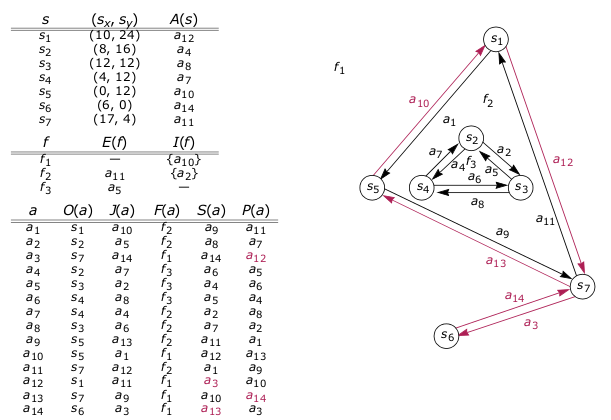
\includegraphics[width=0.8\textwidth]{img/dcel.png}}
    \caption{Exemple de DCEL}
    \label{fig:DCEL}
\end{figure}

\chapter{Paradigmes de construction}

\section{Enveloppe convexe}

\begin{algorithm}[H]
\caption{Recherche de l'enveloppe convexe}
\label{env_convex}
\KwData{Un ensemble $P$ de points du plan}
\KwResult{Une liste $L$ contenant les sommets dans l'ordre horaire}
Supprimer les points identiques\;
Trier les points par coordonnées $x$ croissantes puis $y$ croissantes\;
Mettre les points $p_1$ et $p_2$ dans une liste $L_{sup}$, $p_1$ en premier\;
\For{$i$ = $3..n$}{
    Joindre $p_i$ à $L_{sup}$\;
    \While{$L_{sup}$ contient plus de deux points \textbf{et} les trois derniers points de $L_{sup}$ ne tourne pas à droite}{
        Effacer l'avant-dernier point de $L_{sup}$\;    
    }
}
Mettre les points $p_n$ et $p_{n-1}$ dans une liste $L_{inf}$, $p_n$ en premier\;
\For{$i$ = $n-2..1$}{
    Joindre $p_i$ à $L_{inf}$\;
    \While{$L_{inf}$ contient plus de deux points \textbf{et} les trois derniers points de $L_{inf}$ ne tourne pas à droite}{
    Effacer l'avant-dernier point de $L_{inf}$\;}
}
Effacer $p_n$ et $p_1$ de $L_{inf}$\;
Joindre $L_{inf}$ et $L_{sup}$ pour obtenir $L$\;
\end{algorithm}

L'algorithme \ref{env_convex} est dans la complexité suivante :
\begin{itemize}
    \item $O(n \log(n))$ pour le tri
    \item $O(n)$ pour les deux boucles \textbf{for}
    \item $O(1)$ pour l'effacement dans les listes
\end{itemize}

Au total on a un algorithme en $O(n \log(n)) + O(n)$.

\subsection{Diviser pour régner (\textbf{EC})}

La méthode générale est composé de trois parties :
\begin{enumerate}
    \item Diviser le problème en petite partie
    \item Résoudre chaque partie récursivement (jusqu'au cas trivial)
    \item Fusionner les parties pour obtenir une solution complète
\end{enumerate}

Pour l'enveloppe convexe on pourrait avoir l'algorithme suivant :

\begin{algorithm}[H]
\caption{Enveloppe convexe avec la méthode \textbf{EC}}
\label{ec_env_conv}
\KwData{Un ensemble $P$ de points du plan}
\KwResult{Une liste $L$ contenant les sommets dans l'ordre horaire}
Diviser $S$ par une ligne verticale en deux sous-ensembles $S_1$ et $S_2$\;
Calculer $EC(S_1)$ et $EC(S_2)$\;
Trouver les tangentes supérieures et inférieures (voir figure \ref{fig:ec_env_conv})\;
Fusionner $EC(S_1)$ et $EC(S_2)$\;
\end{algorithm}

Pour l'algorithme \ref{ec_env_conv}, on à la recherche de tangente supérieures et inférieures en $O(n)$. On a donc $T(n) \leq 2\cdot T(\frac{n}{2}) + O(n) \rightarrow O(n \log(n))$.

\begin{figure}
    \centering
    \fbox{
    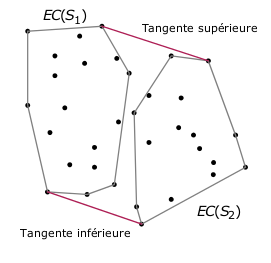
\includegraphics[width=0.4\textwidth]{img/ec_env_conv.png}}
    \caption{Enveloppe convexe avec la méthode de diviser pour régner}
    \label{fig:ec_env_conv}
\end{figure}

\section{Balayage du plan}

Méthode générale :
\begin{itemize}
    \item Commencer avec une structure vide
    \item Remplir une queue de priorité avec des événements-points
    \item Déplacer une ligne de balayage sur tous les objets du plan
    \item Lors de chaque événement, mettre à jour la structure géométrique et la queue d'évé\-nements
\end{itemize}

Paire de point la plus proche en $O(n \log(n))$ et en $O(n)$ pour la mémoire.

\chapter{Intersection de segments de droites}

\chapter{Recherche d'intervalle orthogonaux}

\section{Énumération en $1$ dimension}
Étant donné un ensemble de point dynamique avec une clé, trouver tous les éléments dans l'intervalle $[x,x']$ : utiliser un arbre binaire de recherche $T$ dans lequel on stocke tous les éléments dans les feuilles. Les valeurs des nœuds sont la valeur de l'élément le plus à droite du sous-arbre gauche. \textbf{Solution :}
\begin{itemize}
    \item Partir de la racine avec deux pointeurs
    \item Pour le premier pointeur, si $x <= elt$ descendre à gauche, sinon descendre à droite. Répéter jusqu'à atteindre une feuille.
    \item Pour le deuxième pointeur, si $x' > elt$ descendre à droite, sinon descendre à gauche. Répéter jusqu'à atteindre une feuille.
    \item Depuis le premier pointeur, 
\end{itemize} 

\chapter{Exercices 1}
\paragraph*{1.1} Il n'est pas possible de réaliser ce problème, si on compte le nombre d'intersection total pour chaque segment, on arrive à $5*3=15$, or, lors de chaque intersections, cela rajoute à chaque fois $2$ intersections, donc on arrive jamais à $15$ puisse que $15$ est impair.

Avec $301$ segments qui doivent en couper exactement $201$ autres, cela nous donne $301*201=60501$, c'est impair dont impossible.

Pour résoudre ce problème on peut modéliser sous la forme d'un graphe : $5$ sommets connectés à exactement $3$ autres sommets.

\paragraph*{1.2} Ajouter des nœuds supplémentaires avec un arbre de Steiner, l'arbre de Steiner ce construit à partir du diagramme de Voronoï.

\paragraph*{1.4} Un problème est donnée par une matrice de flot $F$ et une matrice de distance $D$. Si la matrice $D$ est plus grande que $F$ (si il y a plus de place que d'éléments à placer), alors on peut modifier la matrice $F$ avec des éléments quelconque dont le coût est l'élément neutre.

\paragraph*{1.5} $x_i\ in \ \{0,1\}$ avec $\sum i \cdot x_i = 1170$ et $\prod i \cdot (1-x_i) = 36000$ et donc on peut définir la fonction d'utilité $min(|\sum i \cdot x_i - 1170| - |\prod i \cdot (1-x_i) - 36000|)$

\paragraph*{1.6} On peut modéliser ce problème comme un problème de coloration de graphe.

\paragraph*{1.9} 

\chapter{Méthodes constructives}

\section{Construction aléatoire}
Tirer aléatoirement une solution dans l'espace des solutions admissibles. L'avantage est que la méthode est très facile à implémenter mais la qualité de la solution est déplorable et un tirage aléatoire uniforme n'est pas évident à réaliser.

\begin{align*}
& \sigma \text{ : permutation aléatoire } 1..n \\
& \sigma_i \text{ : ième ville visité}\\
& D = (d_{ij})\\
& \text{minimiser } (\sum_{i=1}^{n-1} d_{\sigma_i \sigma_{i+1}}) + d_{\sigma_n \sigma_i}
\end{align*}

ou bien minimiser avec $s_i$ est la ville qui suit la ville $i$
$$
\sum_{i=1}^n d_{i s_i}
$$

\begin{algorithm}[H]
\KwData{Tableau de $n$ element $L$}
\KwResult{Une permutation aléatoire de $L$}
Définir $l$ comme la longueur du tableau\;
\For{i allant de 1 à n}{
    Tirer aléatoirement $j \in [i;n]$\;
    Permuter $L[j]$ avec $L[l]$\;
    $l = l - 1$\; 
}
\end{algorithm}

\section{Méthode gloutonne}

L'idée est de construire une solution élément par élément en ajoutant, à chaque pas, un élément approprié. Cela est optimal pour certain problème.

On part d'une solution $s$ vide ou trivial. On a une fonction de coût incrémental qui mesure empiriquement l'adéquation d'ajouter l'élément $e$ à $s$. Le fait d'ajouter un élément peut ajouter des contraintes sur les prochains éléments à ajouter.

\begin{algorithm}[H]
\tcc*[l]{Algorithme glouton en $O(n^2)$}
\KwData{Une solution partielle minimal $s$ // en général $\emptyset$}
\KwData{$R$ = $E$ // Ensemble des éléments pouvant être ajoutés à $s$}
\KwResult{Une solution gloutonne}

\While{$s$ n'est pas une solution complète}{
    Calculer $c(e,s) \forall e \in R$\;
    Choisir un $e'$ optimisant $c(e,s$)\;
    $s = s \vee {e'}$\;
    \tcp*[l]{propagation des contraintes}
    Supprimer de $R$ tout les éléments qui ne peuvent être ajouter à $s$\;
}
\end{algorithm}

Il existe d'autre algorithme :

\subsection{Regret maximum}
Lors de chaque étape, choisir la ville $e$ qui maximise la fonction
$$
c(s,e) = min_{j,k \in R}d_{je} + d_{ek} - min_{j \in R} d_{ie} + d_{ej}
$$ 

\subsection{Meilleur insertion}
Choisir la ville $e$ qui minimise la fonction
$$
c(s,e) = \text{coût d'insertion minimalde la ville e avec la tournée partiel s}
$$

possible en maximisant : insertion de la ville la plus éloignée. Les deux méthodes sont en $O(n^2)$


\chapter{Méthodes d'amélioration}

Pseudo code d'une méthode d'amélioration locale :

\begin{algorithm}[H]
\tcc*[l]{Trame d'une méthode d'amélioration locale}
\KwData{Une solution donnée (par exemple, à partir d'une construction gloutonne}
\KwResult{Une solution équivalente ou meilleure}
\Do{Une amélioration est effectué}{
    Essayer de trouver une amélioration\;
    Faire l'amélioration trouver\;
}
\end{algorithm}

Exemple de modification :
\begin{itemize}
    \item Remplacer deux arêtes d'une tournée par deux autres
    \item \textbf{2-Opt} : inverser le sens de parcours d'une sous-chaîne (remplacer deux arêtes par deux autres)
    \item \textbf{3-Opt} : déplacer un chemin ailleurs dans la tournée (remplacer trois arcs par trois autres)
    \item \textbf{Or-Opt} : Déplacer une sous-chaîne de $r$ sommet ailleurs dans la tournée avec $r = 3$ puis $2$ puis $1$ etc...
\end{itemize}

\paragraph*{3.1} On arrive deux fois à $-4$ pour le premier chemin améliorant.

\chapter{Méthodes aléatoires}

\section{Choix du prochain élément}

Il existe plusieurs technique pour ce choix :
\begin{itemize}
    \item GRASP : on calcule $c_{min} et c_{max}$ (coût d'insertion) et on choisis l'élément parmis un sous-ensemble $R$ de $E$ où $E$ est l'ensemble des éléments disponibles et $R$ est $\{r \in E | c_{r} \in [c_{min};\alpha(c_{max}-c_{min})]\}$
    \item colonie de fourmie : le choix est inversement proportionnel au coût et les coût sont modifiés en fonction des solutions construites précédemment
    \item technique du bruitage : bruitage du coût en fonction d'une loi
\end{itemize}

\section{Recherches locales aléatoires}

\section{Exercices}

\paragraph*{4.1 : }

\chapter{Méthodes de décomposition}

En général, utiliser pour résoudre des problèmes de très grandes tailles (entre $10^3$ et $10^7$ d'ordre de grandeur).
\begin{itemize}
    \item Jouet : énumération complète
    \item Petit : Méthodes exactes
    \item Moyen : Méta-heuristique (limite de la mémoire en $O(n^2)$)
    \item Grand : Méthode de décomposition
    \item Très grand : Bases de données distribuées
\end{itemize}

\section{Recherche dans de grand voisinage}

Cette technique est applicable typiquement dans un problème de programmation par contrainte avec plusieurs millier de variable. L'idée est de fixée les valeurs de toutes les variables sauf un certain sous-ensemble. On optimise le sous-ensemble et on peut recommencer avec un autre sous-ensemble une fois cela fait.

\section{Popmusic : méthode de décomposition générique}

Idée générale de Popmusic :

\begin{algorithm}[H]
\tcc*[l]{Algorithme Popmusic}
\KwData{Une solution donnée (par exemple, à partir d'une construction gloutonne}
\KwResult{Une solution équivalente ou meilleure}
\For{Chaque sous-ensemble de la solution}{
    Optimiser le sous-ensemble\;
}
\end{algorithm}

La difficulté est que les sous-ensemble ne sont peut-être pas indépendant les uns des autres.

\begin{algorithm}[H]
\tcc*[l]{Algorithme plus précis pour Popmusic}
\KwData{Une solution $S = s_1 \vee s_2 \vee ... \vee s_p$}
\KwData{$O = \emptyset$}
\KwResult{Une solution équivalente ou meilleure}
\While{$S \neq O$}{
    Choisir un élément $S_i \notin O$\;
    Créer un sous-problème $R$ composée de $r_i \in S$ les plus proches de $s_i$\;
    Optimiser $R$\;
    \eIf{$R$ est amélioré}
        {$O \leftarrow O \setminus R$}
        {$O \leftarrow O \vee s_i$}
}
\end{algorithm}

\begin{algorithm}[H]
\tcc*[l]{Grand voisinage pour le VRP}
\KwData{Une solution $S$ initial}
\KwResult{Une solution équivalente ou meilleure}
 partir de $S$, supprimer $n$ point de la solution\;
Réinsérer les clients au mieux\; 
\end{algorithm}

\subsection{Popmusic pour la classification non-supervisée}

Les parties sont les éléments d'une même classe, on calcule la dissimilarité moyenne entre les éléments de classes différentes et la distance entre les centroïdes, puis on optimise la solution en déplacement progressivement des centres et on recalcule le tout avec l'algorithme K-means.

\subsection{Compression d'image par quantification de vecteur}

On cherche à décomposer une image en blocs de $b$ pixels (par exemple $b=5 \times 3$). On cherche à trouver la meilleur palette de $2^k$ couleurs, vues comme des vecteurs de $3 \times b$ octets. Il s'agit d'un problème de classification composer de millions d'éléments en des milliers de groupes. On code chaque bloc par $k$ bits.

\section{Exercices}

\paragraph*{5.1 : } 

\paragraph*{5.2 : } 

\chapter{Fourmis artificielles et constructions aléatoires}

\begin{algorithm}[H]
\caption{Système de fourmis pour le TSP}
\KwData{Une matrice de distance entre les villes $D=(d_{ij} = \frac{1}{\eta_{ij}})$}
\KwData{Une matrice de trace $T=(\tau_{ij})$}
\KwData{Les paramètres $\alpha$, $\beta$, $\rho$, $\tau_0$, $Q$ et $max\_iter$}
\KwResult{Une solution}
Initialisation : Poser $\tau_{ij} = \tau_0$\;
\For{$max\_iter$ itérations}{
    $R = (r_{ij}) = 0$\tcp*[r]{Renforcement des arêtes}
    \For{$k = \{1,...,m\}$}{
        $L = 0$\;
        Choisir une ville $i$ au hasard\;
        \While{Toutes les villes ne sont pas visité}{
            Choisir une ville $j$ non-visitée avec $P$ proportionnelle à $\tau_{ij}^\alpha \cdot \eta_{ij}^\beta$\;
            $L = L + d_{ij}$\;
            $i=j$\;
        }
        \For{tout les trajets $(i,j)$ de la tournée}{
            $r_{ij} = r_{ij} + Q / L$
        }
    }
    $T = (1-\rho)T + R$\tcp*[r]{Mise à jour des traces de phéromones}
}
\end{algorithm}

\chapter{Recherche avec tabous}

Il s'agit d'une recherche locale avec la politique du meilleur mouvement sauf qu'elle possède certain ajout :
\begin{itemize}
    \item Interdire de revenir à une solution déjà visité
    \item Interdire d'effectuer l'inverse d'un mouvement
    \item Pénaliser les mouvements fréquemment utilisés
    \item Forcer l'utilisation de mouvement jamais utilisés
    \item Lever une interdiction après un certain nombre d'itérations
\end{itemize}

Besoins :
\begin{itemize}
    \item Une fonction d'aspiration : un mouvement interdits, qui améliore $s^*$, est accepté
    \item Intensification de la recherche : diminuer le nombre de mouvement interdits et repartir depuis la meilleure solution trouvée
    \item Diversification de la recherche : Fréquence des mouvements utilisés, mémoire des bonnes solutions (Chemin de liaison, construction de vocabulaire)
\end{itemize}

\begin{algorithm}[H]
\caption{Recherche avec tabous de base}
\KwData{Solution initiale $s$}
\KwData{Fonction utilité $f$ à minimiser}
\KwData{Ensemble $M$ des mouvements applicables à toute solution}
\KwData{Paramètres $t$(durée des interdictions), $max\_iter$}
\KwResult{Une solution équivalente ou meilleure}
Initialisation : $T = \emptyset$, $s^* = s$\;
\For{$max\_iter$}{
    meilleur\_voisin = $\infty$\;
    \For{$m\in M$, $m \notin T$}{
        \If{meilleur\_voisin $> f(s \oplus m)$}{
            meilleur\_voisin $= f(s \oplus m)$\;
            meilleur\_mouvement $= m$\;
        }
        $s = s \oplus $ meilleur\_mouvement\;
        Remplacer dans $T$ le plus ancien mouvement par $meilleur\_mouvement^{-1}$\;
        \If{meilleur\_voisin $< f(s^*)$}{
            $s^* = s$\;
        }
    }
}    
Retourner $s^*$\;
\end{algorithm}

\section{Recherche avec tabous pour le QAP}
Une solution est une permutation $p$ de $n$ éléments. Mouvement applicable à n'importe quelle : Transposer les objets $i$ et $j$ $(m=(i,j),1\leq i < j\leq n)$. C'est à dire : l'objet $i$ actuellement en position $p_i$ est déplacé en position $p_j$ et l'objet $j$ est déplacé en $p_i$.

Inverse d'un mouvement : replacer simultanément l'objet $i$ en $p_i$ et l'objet $j$ en $p_j$.

Mémoire : 
\begin{itemize}
    \item Matrice $T=t_{ir}$ de taille $n\times n$
    \item $t_{ir}$ numéro d'itération où l'on peut à nouveau placer l'objet $i$ en position $r$
    \item Le mouvement $(i,j)$ est interdit à la solution $p$ à l'itération $k \Longleftrightarrow (t_{ip_j} > k) \wedge (t_{jp_i} > k)$
    \item Le statut d'un mouvement $(i,j)$ peut être tester en temps constant
\end{itemize}

\section{Durée des interdictions}
La durée des interdictions influence énormément l'évolution de l'algorithme, si la durée est trop faible, on risque de revenir sur ses pas, faire des cycles ou encore d'être piéger dans un optimum local. Au contraire, si elle est trop grande, il y aura un nombre limité de mouvement réalisable et on risque fortement de ne pas voir "les bon chemins" car tout le temps une partie est interdite.

Solutions :
\begin{itemize}
    \item Apprendre dynamiquement la durée des inter\-dictions (augmenter la durée des inter\-dictions si on visite 2 fois la même solution, diminuer la durée si on ne visite pas la même solution pendant un plusieurs itérations)
    \item Tirer aléatoirement la durée des interdictions : des mouvements sont interdits pendant longtemps mais la plupart sont juste inaccessible pendant un court instant
\end{itemize}

\section{Mémoire à long terme}
\paragraph*{Pénalité sur les fréquences : }Le but est d'éviter les mouvements de faibles coût en mémo\-risant la fréquence d'utilisation de chaque mouvement et en pénalisant de $F\cdot freq(m)$ le mouvement $m$.
\paragraph*{Recherche locale guidée : } Lorsqu'un optimum local est atteint, l'élément le plus couteux de la solution est pénalisé pour défavoriser sont utilisation future.
\paragraph*{Forcer des mouvements : } Casser la structure d'une solution en identifiant les mouvements jamais choisis durant les $K$ dernières itérations. Pour QAP, on lit cela directement dans la matrice $T$.

\chapter{Algorithmes génétiques, recherche par dispersion et essaims particulaires}

\section{Population de solution}
Il est facile d'obtenir beaucoup de solution différentes pour un problème. L'idée est de construire de nouvelle solutions précédemment obtenues et de disperser les solutions générées dans tout l'ensemble des solutions. On suppose que la combinaison des solutions peut sélectionner les bonnes caractéristiques de chacune.

\section{Algorithmes évolutionnaires}
Darwin : les êtres humains transmettes des caractéristiques utiles à leurs enfants. Le néo-darwinisme : la mutation génétique.

\begin{center}
    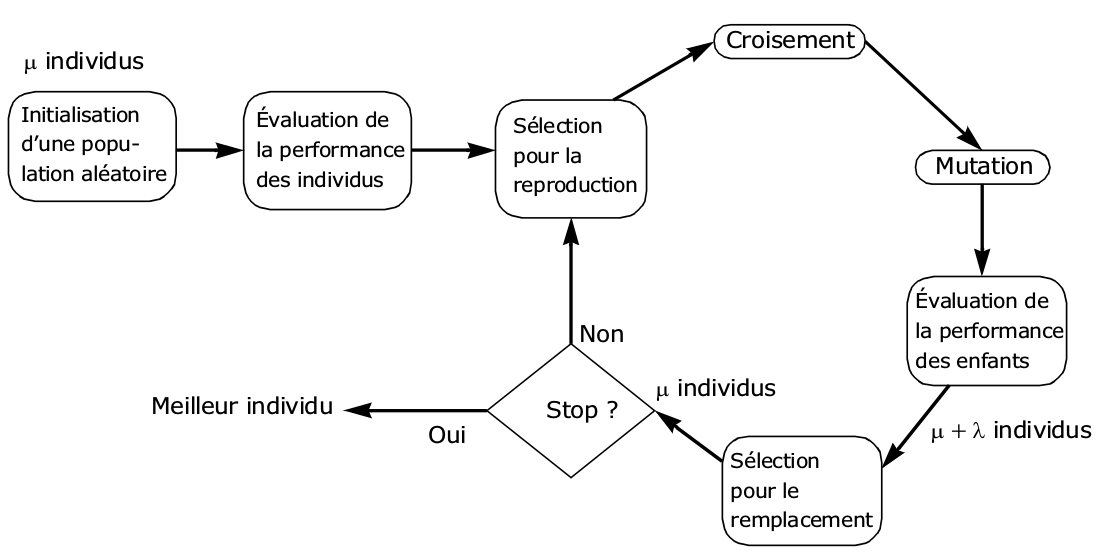
\includegraphics[width=0.9\textwidth]{img/schema.png}
\end{center}

\begin{algorithm}[H]
\caption{Générer une population de $\mu$ solutions}
\Repeter{Jusqu'à ce qu'un critère d'arrêt soit satisfait}{
    Sélectionner des solutions pour la reproduction (parents)\;
    Combiner des solutions pour obtenir $\lambda$ enfants provisoires\;
    Appliquer un opérateur de mutation/réparation à chaque enfant\;
    Évaluer la performance de chaque enfant\;
    Parmi la population complète, sélectionner $\mu$ solutions pour la prochaine population\;
}
\end{algorithm}

\subsection{Sélection aléatoire}

\paragraph*{La roulette : } On attribue à chaque individu une valeur de performance, on somme toutes ces valeurs et on tire au hasard un nombre entre $0$ et cette valeur pour tomber sur l'élément à sélectionner.

\paragraph*{Échantillonnage stochastique universel : } On tire à intervalle régulier chaque individu (on peut tomber deux fois sur le même !).

\paragraph*{Rang : } On trie les solutions et on calcule le rang $r$ de l'individu choisi : $r = \mu \cdot (1-\sqrt[P]{U(0.1)})$ ($U(n,m)$ tire un nombre au hasard entre $n$ et$m$), avec :
\begin{itemize}
    \item $p=1$ : sélection aléatoire uniforme
    \item $p>1$ : les meilleurs individu sont favorisés
\end{itemize}

\subsection{Opérateurs de croisement génétique uniforme}
Les solutions sont représentées par des vecteurs de taille donnée. On tire aléatoirement les composantes des nouvelles solutions, les "enfants" en copiant aléatoirement les composantes des deux parents.

Le croisement peut être partiel (par exemple si le vecteur doit respecter la contrainte que les éléments sont une permutations des nombres de $1$ à $n$).

\paragraph*{Croisement par vecteur : } On coupe en $1$, $2$, ... et on prend l'un ou l'autre pour chaque partie de l'enfant.

\paragraph*{Opérateur OX : } respect des sous-séquences : on prend une sous-séquence et on recopie, à la suite, les éléments non pris.

\subsection{Opérateurs de mutation}
Vecteurs $(0-1)$ : modifier chaque bit aléatoirement avec la même probabilité. Modifier un nombre donné de bits aléatoirement.

\subsection{Gestion de la population}:

\begin{itemize}
    \item \textbf{Remplacement générationnel} : Seules les enfants survivent d'une génération à l'autre ($\lambda = \mu$).
    \item \textbf{Stratégie évolutionnaire} : Seuls les $\mu$ meilleur enfants sont conservés ($\lambda > \mu$).
    \item \textbf{Remplacement stationnaire} : Remplacer aléatoirement $\lambda$ parents par des enfants ($\lambda$ est petit (1 ou 2)).
    \item \textbf{Stratégie élitiste} : De la population complète $\lambda + \mu$ on ne conserve que les $\mu$ meilleurs.
\end{itemize}

Plus une population est grande implique :
\begin{itemize}
    \item Une plus grande diversité
    \item Des meilleurs solutions sont obtenus après convergence
    \item Un taux de convergence plus lent et de plus grand temps de calcul
\end{itemize}

\section{Recherche par dispersion}

\begin{algorithm}[H]
\caption{Recherche par dispersion}
\Repeter{Jusqu'à ce qu'un critère d'arrêt soit satisfait}{
    Créer une population diversifié\;
    Améliorer/réparer toutes les solutions de la populations\;
    Sélectionner un ensemble de référence avec des solutions diversifiées et élites\;
    \Repeter{L'ensemble de référence est modifié}{
        \For{Chaque sous-ensembles de l'ensemble de référence}{
             Combiner les solutions du sous-ensemble\;
             Améliorer/réparer la solution combiné\;
             Inclure la nouvelle solution dans la population\;        
        }
        Mettre à jour l'ensemble de référence (conserver les solutions les meilleurs et les plus diversifiées)
    }
}
\end{algorithm}

\begin{algorithm}[H]
\caption{GRASP-PR}
    Générer une population de $\mu$ solutions différentes avec une recherche gloutonne randomisée et une recherche locale\;
    \Repeter{jusqu'à ce qu'un critère d'arrêt soit satisfait}{
        Générer une nouvelle solution $s$ avec une recherche gloutonne randomisée et une recherche locale\;
        Sélectionner une solution aléatoire $s'$ dans la population\;
        Effectuer un chemin de liaison entre $s$ et $s'$\;
        \If{la meilleur solution $s^*$ trouvée sur le chemin est meilleur qu'une certaines solutions de la population}{
            $s^*$ remplace une solution de la population plus mauvaise que $s^*$\;       
        }
    }
\end{algorithm}

\section{Méthodes à particules}

Une particule est une solution (en principe un vecteur $x$ de réels (position)). Les particules ont des interactions entre elles, elles n'en créent pas d'autres.

La particule $i$ est attirée par une force $f_{ij}$ vers la particule $j$. Les particules ont une vitesse et éventuellement une charge électrique. La nouvelle position d'une particule dépend de la force qui s'applique sur elle.

\begin{algorithm}[H]
\DontPrintSemicolon
\caption{Méthodes à particules}
    Générer une position aléatoire $x_i$ pour chaque particule\;
    \tcp*[l]{Pour les essaims particulaires : $+$ un vecteur de vitesse}
    \Repeter{jusqu'à ce qu'un critère d'arrêt soit satisfait}{
        \For{Chaque particule $i$}{
            Effectuer une recherche locale\;
            Calculer les forces $f_{ij}$\;
            Déplacer $i$ dans la nouvelle position $x_i$\;        
        }
    }
\end{algorithm}

\section{Exercices}

\paragraph*{8.1 : } Si on code un binaire on a des problèmes si on croise des nombres proches, par exemple 127 et 128. Solution : prendre un code de Gray.

\paragraph*{8.2 : } $(4,2,3,0,1,0)$ : $(4,6,2,5,1,3)$, $(0,0,3,1,2,0)$ : $(1,2,,,4,3)$... impossible. À l'élément $i$, on doit avoir un nombre plus petit ou égale à $n-i$.

\end{document}
